\chapter{Sparsity Tracing via NaN-Propagation}
\label{sec:nan_propagation}

A key challenge in applying code transformations is handling external black-box (i.e., non-traceable) function calls within the analysis graph. While code transformations can apply techniques like automatic differentiation and automated sparsity detection to accelerate traceable code, these efficiency gains are lost when opaque black-box functions are present. Here, gradient calculation methods must invariably fall back to slower techniques, such as finite-differencing or complex-step derivative computation \cite{martins_complexstep_2003}. Thus, this workaround to patch a black-box model into a code-transformations-based MDO tool using simple finite-differencing usually leads to poor performance.

To break down this problem, we can ask ourselves what the minimum amount of information needed to achieve meaningful acceleration on black-boxes would be. In an ideal case, we would like to have a fast way to directly evaluate the Jacobian of the black-box function at some given point in the input space. This is, however, not possible in the general case of a black-box function, where the only guaranteed way of interacting with the function is via inputs and outputs.

The next-best option would be to obtain information that allows us to compute the Jacobian more efficiently using finite-differencing. One example of such information is the sparsity pattern of the Jacobian of the black-box function. This sparsity pattern essentially gives a map of which inputs have the potential to affect each output. Armed with this information, we can perform Jacobian compression via coloring \cite{gebremedhin_efficient_2009, gebremedhin_what_2005}. This allows the Jacobian to be calculated with fewer function evaluations, even in the case of simple finite-differencing.


\section{Existing Approaches}
\label{sec:nan-existing-methods}

Currently, the most common approach to obtain the sparsity pattern of a black-box function is to first construct the (dense) Jacobian, evaluated at some particular point in the input space that is assumed to be representative. (In the context of an optimization framework, this input point usually corresponds to the initial guess.) This Jacobian is then evaluated, often by finite-differencing. Then, a critical assumption is made: it is assumed that any zero entries in this evaluated Jacobian are indicative of a zero entry in the true Jacobian -- in other words, sparsity seen at one point indicates sparsity at all points. Due to this assumption, the sparsity pattern constructed with this method is only an estimate, not a guarantee.

The fact that this reconstructed sparsity pattern is only an estimate is inevitable for black-box functions. To illustrate why, consider a piecewise function, where input $x_j$ influences output $y_i$ when $x_j$ is within a certain interval but not outside of it. It is possible to construct a pathological function where this region of influence is arbitrarily small, such that it will nearly never be detected by direct sampling of the Jacobian. Such cases will result in a \emph{false negative} in the estimated sparsity pattern: cases where $x_j$ and $y_i$ are believed to be independent, when in reality they are not.

This kind of branching code execution is perhaps the most common cause of such false negatives (often via conditional expressions) in the context of engineering analysis. However, there are other relevant failure modes as well. One possible cause of false negatives is if the representative input point yields a partial derivative of zero only due to coincidence, rather than due to mathematical structure. One simple illustrative example is the function $f(x) = x^2$, if the evaluation point of $x = 0$ is chosen. Here, a central finite difference will see zero gradient and incorrectly infer no dependency. On most functions of practical interest, such points are usually rare within the input space\footnote{In most practical functions $\vec{f}(\vec{x}): \R^m \rightarrow \R^n$, the dimensionality of all manifolds where $\partial f_i/\partial x_j=0$ is less than the dimensionality of the input $\vec{x}$. In such cases, \emph{almost all} points will be free of coincidental zeros.}. However, in an optimization context, the distribution of user-specified initial guesses is not uniform, and in fact adversarial: users will preferentially supply near-optimal initial guesses, which have near-zero gradients (if the problem is unconstrained). Because of this, this effect can contribute to a non-negligible rate of false negatives in practice.

\emph{False positives}, where $x_j$ and $y_i$ are believed to be related when they are not, are also possible, though rarer. A practical example where this could occur is with a black-box function that has truncation error, perhaps due to a nonlinear solver or numerical integrator that uses a value-dependent convergence criteria. In such cases, changing one input may alter the number of iterations required for convergence. This can cause changes in the truncation error of all outputs—even those that are mathematically-unrelated to that input. Thus, changes in this truncation error (i.e., a differing number of iterations) may yield a nonzero Jacobian entry, even if the math that the code aims to represent has no such dependency. Other false positive scenarios, such as stochastic functions, are possible but relatively uncommon in engineering analysis. In either the false-negative or false-positive case, an interesting observation is that the sparsity of the function \emph{in code} may not match the sparsity of the mathematical model the code aims to represent.

For reasons related to Jacobian compression (described later via demonstration in Section TODO), the harm caused by a false-negative and a false-positive are far from equal. The ultimate effect of a false-positive is that subsequent gradient calculations will be slightly slower—though still numerically correct. On the other hand, the ultimate effect of a false-negative is that gradient calculations can be incorrect. Worse yet, these incorrect results can occur silently — in the context of design optimization, an incorrect gradient might only be detected much later in the development effort, when an optimizer consistently cannot converge (as the KKT conditions cannot be satisfied). By this point in the design process, the combined optimization model is usually much more complex, and finding and eliminating an incorrect-gradient error becomes enormously tedious. Because of this, a new method for black-box sparsity estimation that eliminates false-negative failure modes offers significant value to the end-user, even if it comes at the cost of false-positive failure modes. In other words, the focus of black-box sparsity estimation within this context should be to build up a \emph{conservative} estimate of the sparsity pattern that trades away specificity in favor of sensitivity.


\section{NaN-Propagation Overview and Demonstration}
\label{sec:nan-demo}

In this chapter, we present a novel technique for generating these conservative estimates of the sparsity pattern of black-box functions. As a high-level comparison against the existing technique described in this section, this proposed new technique:

\begin{itemize}[noitemsep]
    \item Eliminates a false-negative failure mode, namely coincidental zero gradients.
    \item Adds a new false-positive failure mode, for functions with internal mathematical cancellation.
    \item Is either equivalent in runtime speed, or potentially much faster due to \emph{short-circuiting operators}. This consideration is primarily determined by behavior of the math library used by the black-box function.
    \item Is compatible with most black-box functions, but not all, due to possible internal handling of NaN values. However, this incompatibility is usually easily and immediately detected, allowing the user to fall back to the existing technique.
\end{itemize}

This new technique, and these three high-level tradeoffs, are the focus of the following section.


This thesis contribution introduces a novel technique that we call \textit{NaN propagation} to trace these input-output dependencies through black-box functions. The name refers to ``not-a-number'' (NaN), which is a special value in floating-point arithmetic that is often used to represent undefined, missing, or otherwise unrepresentable values. The proposed technique exploits the fact that Not-a-Number (NaN) values are universally propagated through floating-point numerical computations; colloquially, they tend to ``contaminate'' any calculation that is given a NaN input. For example, a dyadic operation with a just one NaN operand will return NaN. This behavior is explicitly part of math library APIs that follow the IEEE 754 standard \cite{ieee754}, first established in 1985. Because nearly all floating-point math libraries created since the advent of IEEE 754 follow it, this presents a fascinating way to potentially trace sparsity in a way that is essentially independent of math library or programming language. By systematically contaminating inputs to a black-box function with NaN values and observing which outputs become NaN, an estimate of the sparsity pattern can be reconstructed.

\subsection{Example Black-Box Function: Wing Weight Model in TASOPT}

Some of the more nuanced details of the proposed NaN-propagation technique are most clearly explained through demonstration. To do this, we leverage one of the constituent submodels within \emph{TASOPT}, an aircraft design optimization suite for tube-and-wing transport aircraft developed by Drela \cite{drela_tasopt_2010}. The submodel we use is a wing weight model \footnote{In TASOPT, this model is named \texttt{surfw}.}, with the major modeling considerations shown in Figure \ref{fig:nan-tasopt-wing-weight}. The model is relatively detailed, with 38 inputs and 37 outputs. Inputs include geometric parameters, material properties, and configuration-level decisions (e.g., the number and location of engines, or the presence and dimensions of a strut). Outputs are the weights of various wing components, metrics describing the weight distribution, stresses at key points, and other quantities of interest.

\begin{figure}[H]
    \centering
    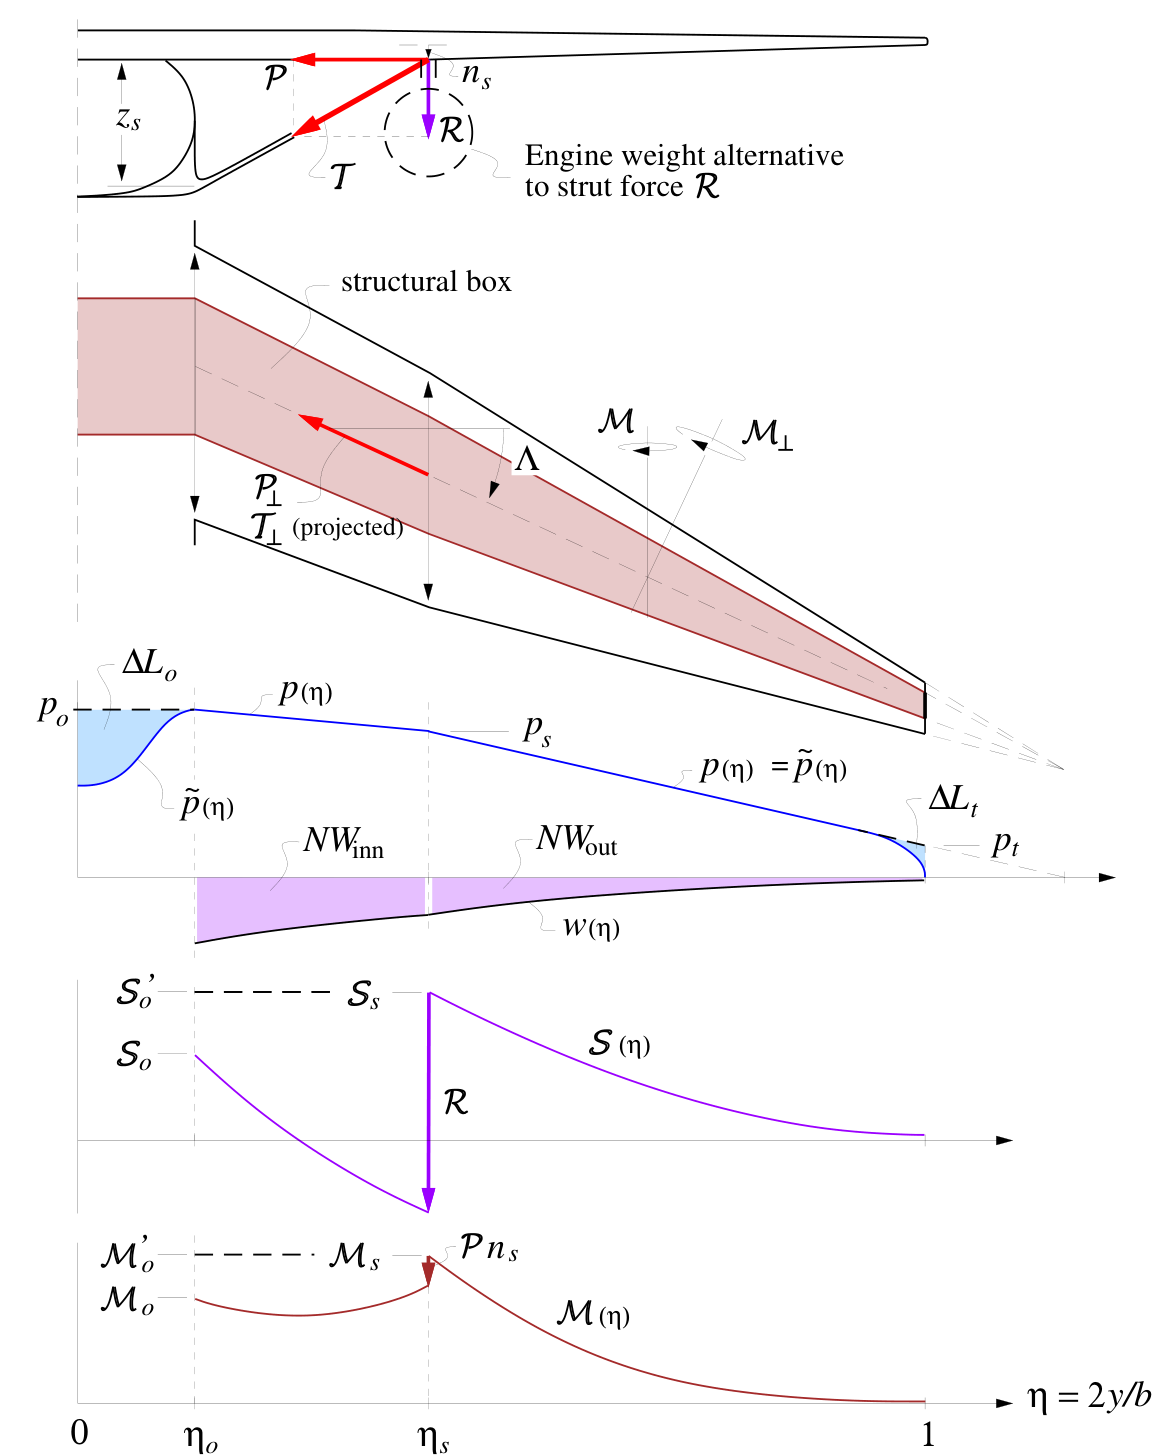
\includegraphics[width=4in]{../figures/nan-propagation/image1.png}
    \caption{Illustration of TASOPT's wing weight model, reproduced from Drela \cite{drela_tasopt_2010}. The model uses an Euler-Bernoulli beam model to compute shear and moment distribution, and accepts a relatively large set of geometric parameters as inputs.}
    \label{fig:nan-tasopt-wing-weight}
\end{figure}


For the purposes of this demonstration, the code implementation of this model is accessed through \emph{TASOPT.jl}, which is a transpilation of the original Fortran code into Julia performed by Prakash et al. \cite{tasopt_jl}. We aim to estimate the sparsity pattern of this function from within Python while accessing this model only through a Python-Julia interface, making this a true black-box function written in an entirely separate programming language.

\subsection{Sparsity Evaluation}

The first step in the NaN-propagation technique is to obtain a representative input. In the context of an optimization problem, the initial guess provides a natural choice:

\begin{figure}[H]
    \centering
    \includegraphics[page=2, width=5in]{../figures/nan-propagation/cropped.pdf}
\end{figure}

Next, we create a set of ``contaminated'' inputs, essentially by merging this input with one-hot encoded NaN values:

\begin{figure}[H]
    \centering
    \includegraphics[page=3, width=5in]{../figures/nan-propagation/cropped.pdf}
\end{figure}

Finally, we evaluate the black-box function at each of these contaminated inputs, and observe which outputs become NaN. For example, the output for one such contaminated input is shown below:

\begin{figure}[H]
    \centering
    \includegraphics[page=4, width=5in]{../figures/nan-propagation/cropped.pdf}
\end{figure}

This simple procedure yields the complete bipartite graph of which inputs and outputs are linked, and this can be interpreted as a sparsity pattern. For the demonstration case study, the sparsity pattern is shown in Figure \ref{fig:nan-jacobian}.

\begin{figure}[H]
    \centering
    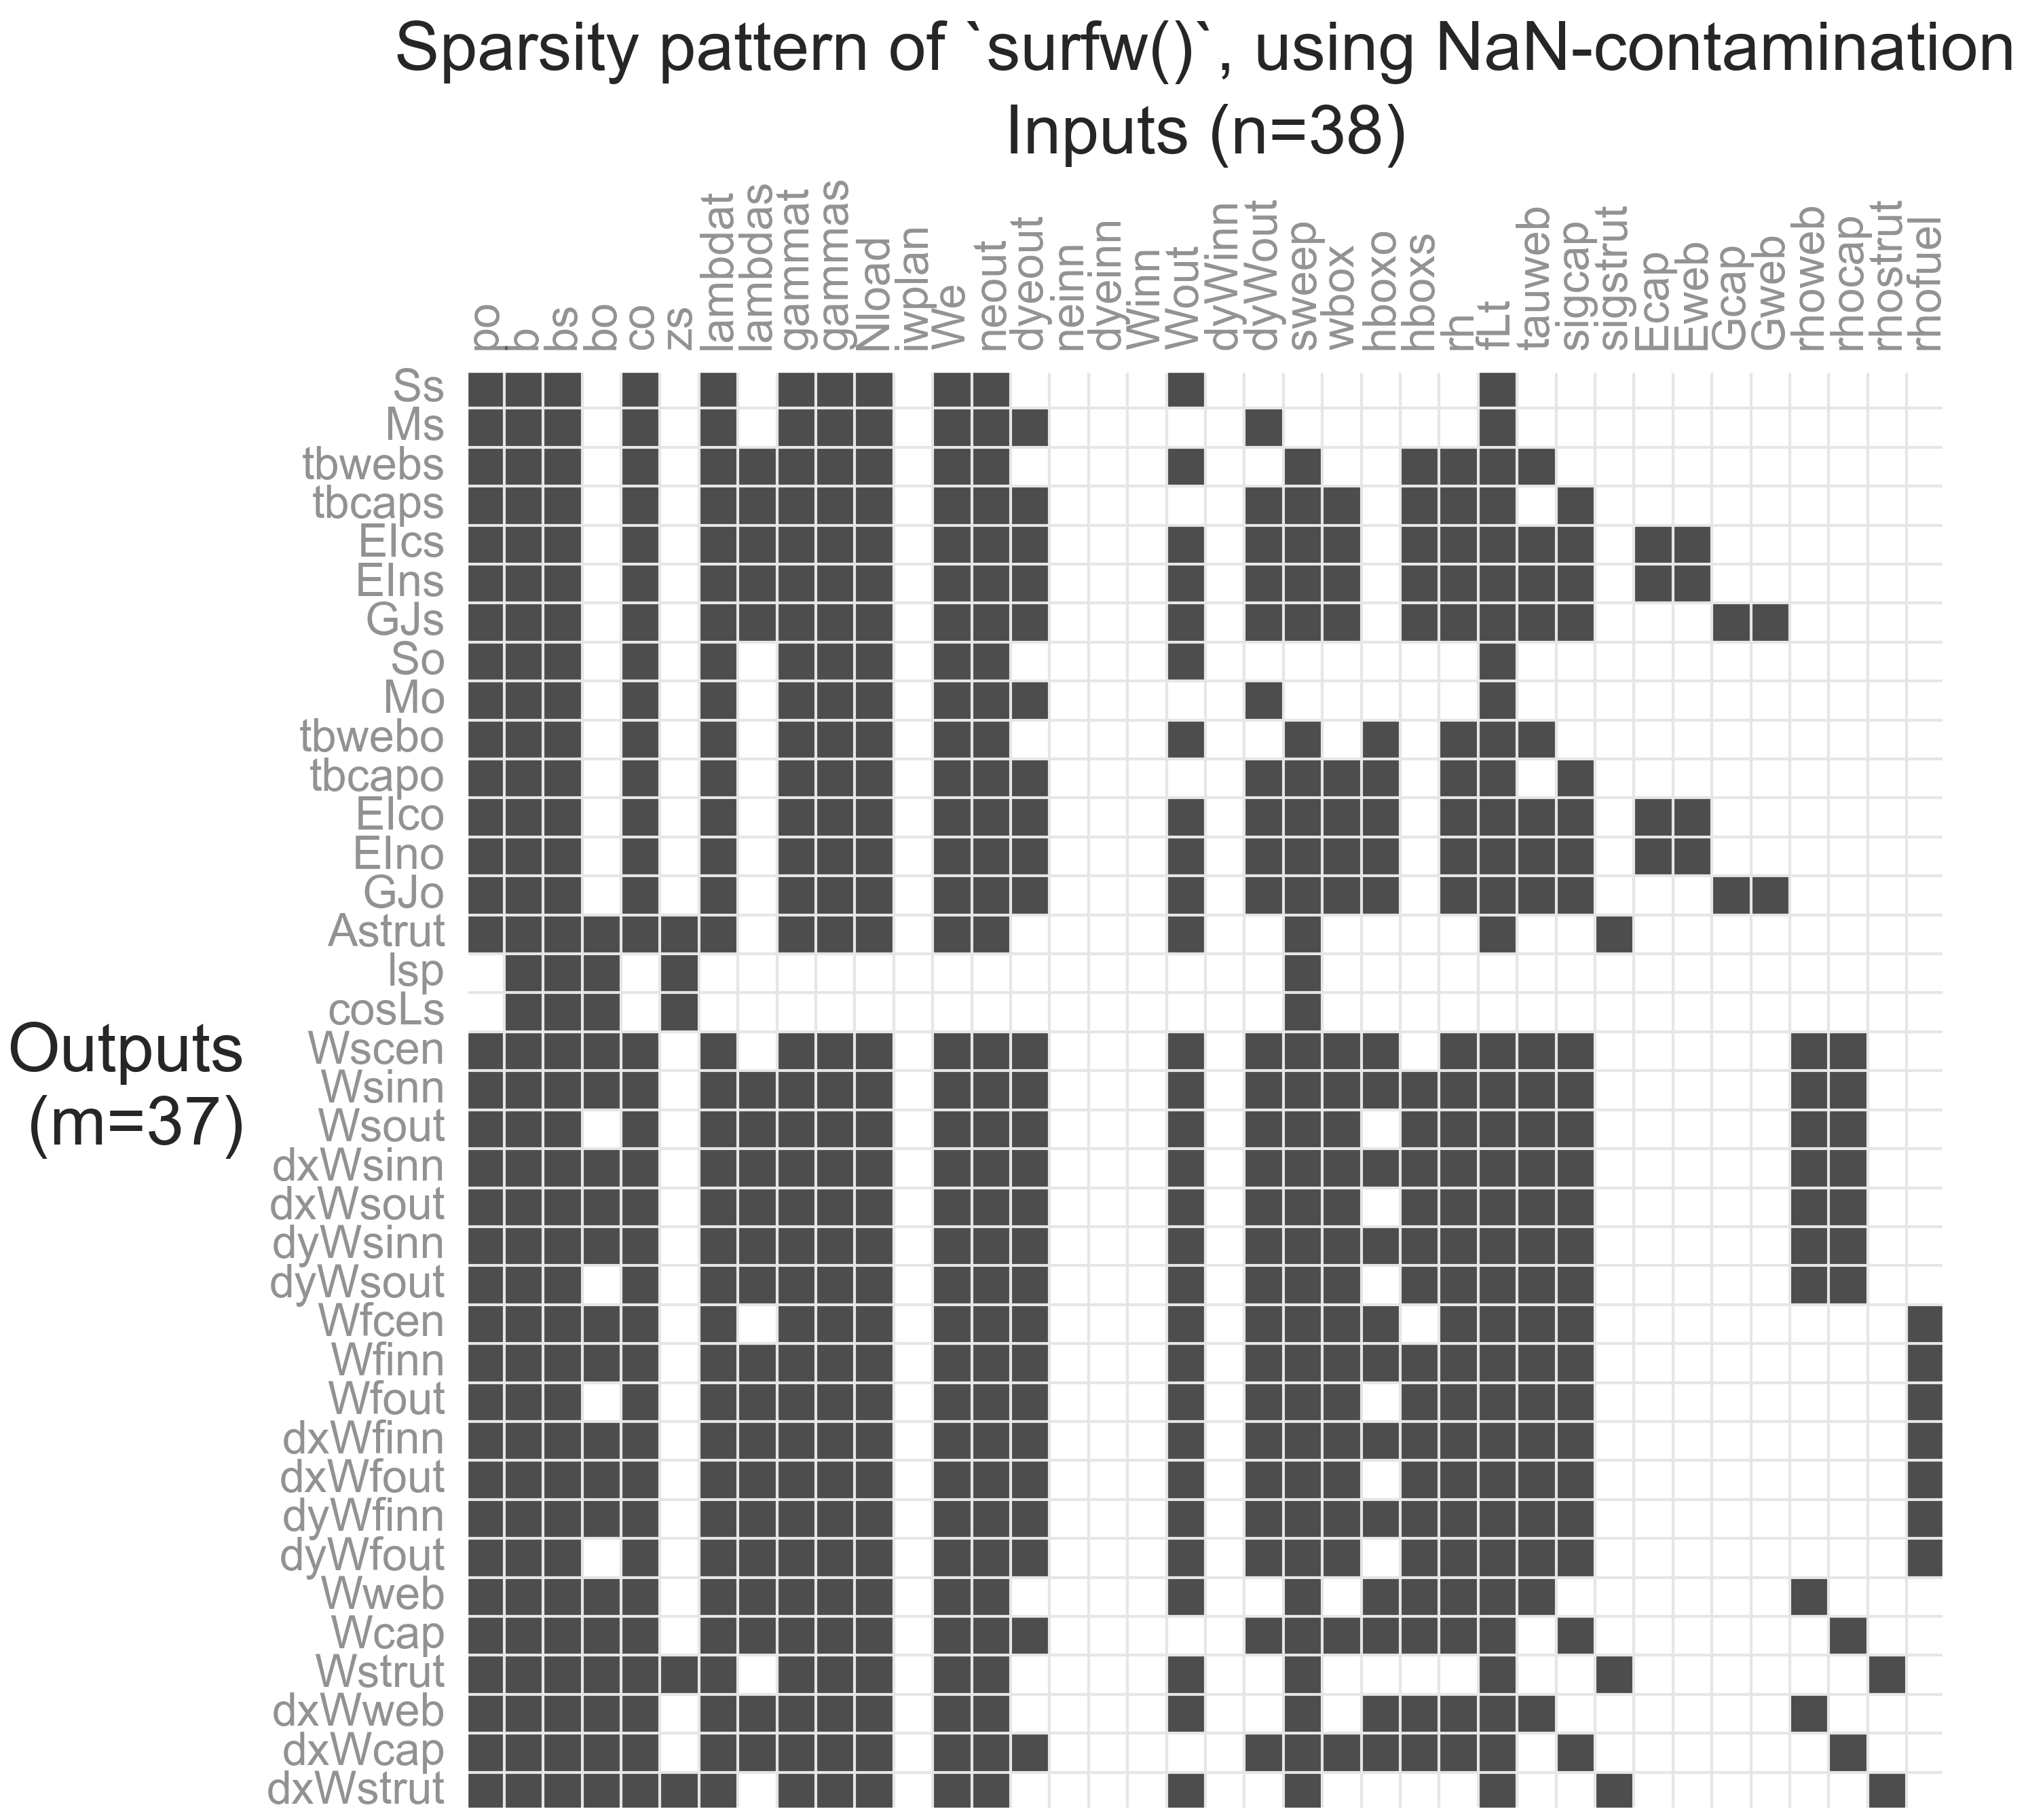
\includegraphics[width=6in]{../figures/nan-propagation/image2-crop.png}
    \caption{Sparsity pattern of the TASOPT wing weight model, estimated using NaN propagation. In this visualization, gray squares indicate nonzero entries in the Jacobian, }
    \label{fig:nan-jacobian}
\end{figure}

A key result is that this NaN-contamination technique eliminates the possible false-negative failure mode of coincidental zero gradients that can occur with existing gradient-based methods. Consider the example case discussed in Section \ref{sec:nan-existing-methods}, where the sparsity of the function $f(x) = x^2$ is traced at $x=0$. Here, a NaN-contamination technique will still detect the dependency between $x$ and $f(x)$, while existing methods will not. Because the potential consequence of a false-negative is so large, this represents a significant advantage over existing methods.

\subsection{Jacobian Compression}

This sparsity pattern can be used to enable gradient computation accelerations via simultaneous evaluation. More precisely, this involves Jacobian compression across columns, since the gradients of this black-box will later be obtained with finite-differencing (``forward-mode''-like behavior). Briefly, the steps to achieve this are:

\begin{enumerate}
    \item Convert the sparsity pattern into an undirected graph representation where each node corresponds to an input (i.e., a column in Figure \ref{fig:nan-jacobian}), and the presence of each edge indicates that the corresponding pair of inputs has overlapping sparsity. Conveniently, the adjacency matrix of this graph can be obtained by computing the Gramian of the sparsity pattern. If the sparsity pattern is represented as the binary matrix $S$, then the adjacency matrix of the graph is the binary matrix $S^T S \neq 0$.
    \item Apply a vertex coloring algorithm to this graph. This is a well-studied problem with many efficient approximate algorithms available \cite{kubale_graph_2004}.
\end{enumerate}

Visually, the result of this process can be shown with the compressed Jacobian of Figure \ref{fig:nan-jacobian-compressed}. Here, several columns show a combination of multiple inputs, and gradients with respect to these inputs can be safely computed simultaneously due to structural independence. The improvement in gradient computation speed is case-dependent, but in this demonstration, a reduction from 38 inputs to 25 effective inputs is achieved. Because gradient computation runtime scales linearly with the number of inputs in a finite-difference (or complex-step) context, this means that all future gradient calculations are roughly $38/25 \approx 1.52$x faster than a dense Jacobian construction.

\begin{figure}[H]
    \centering
    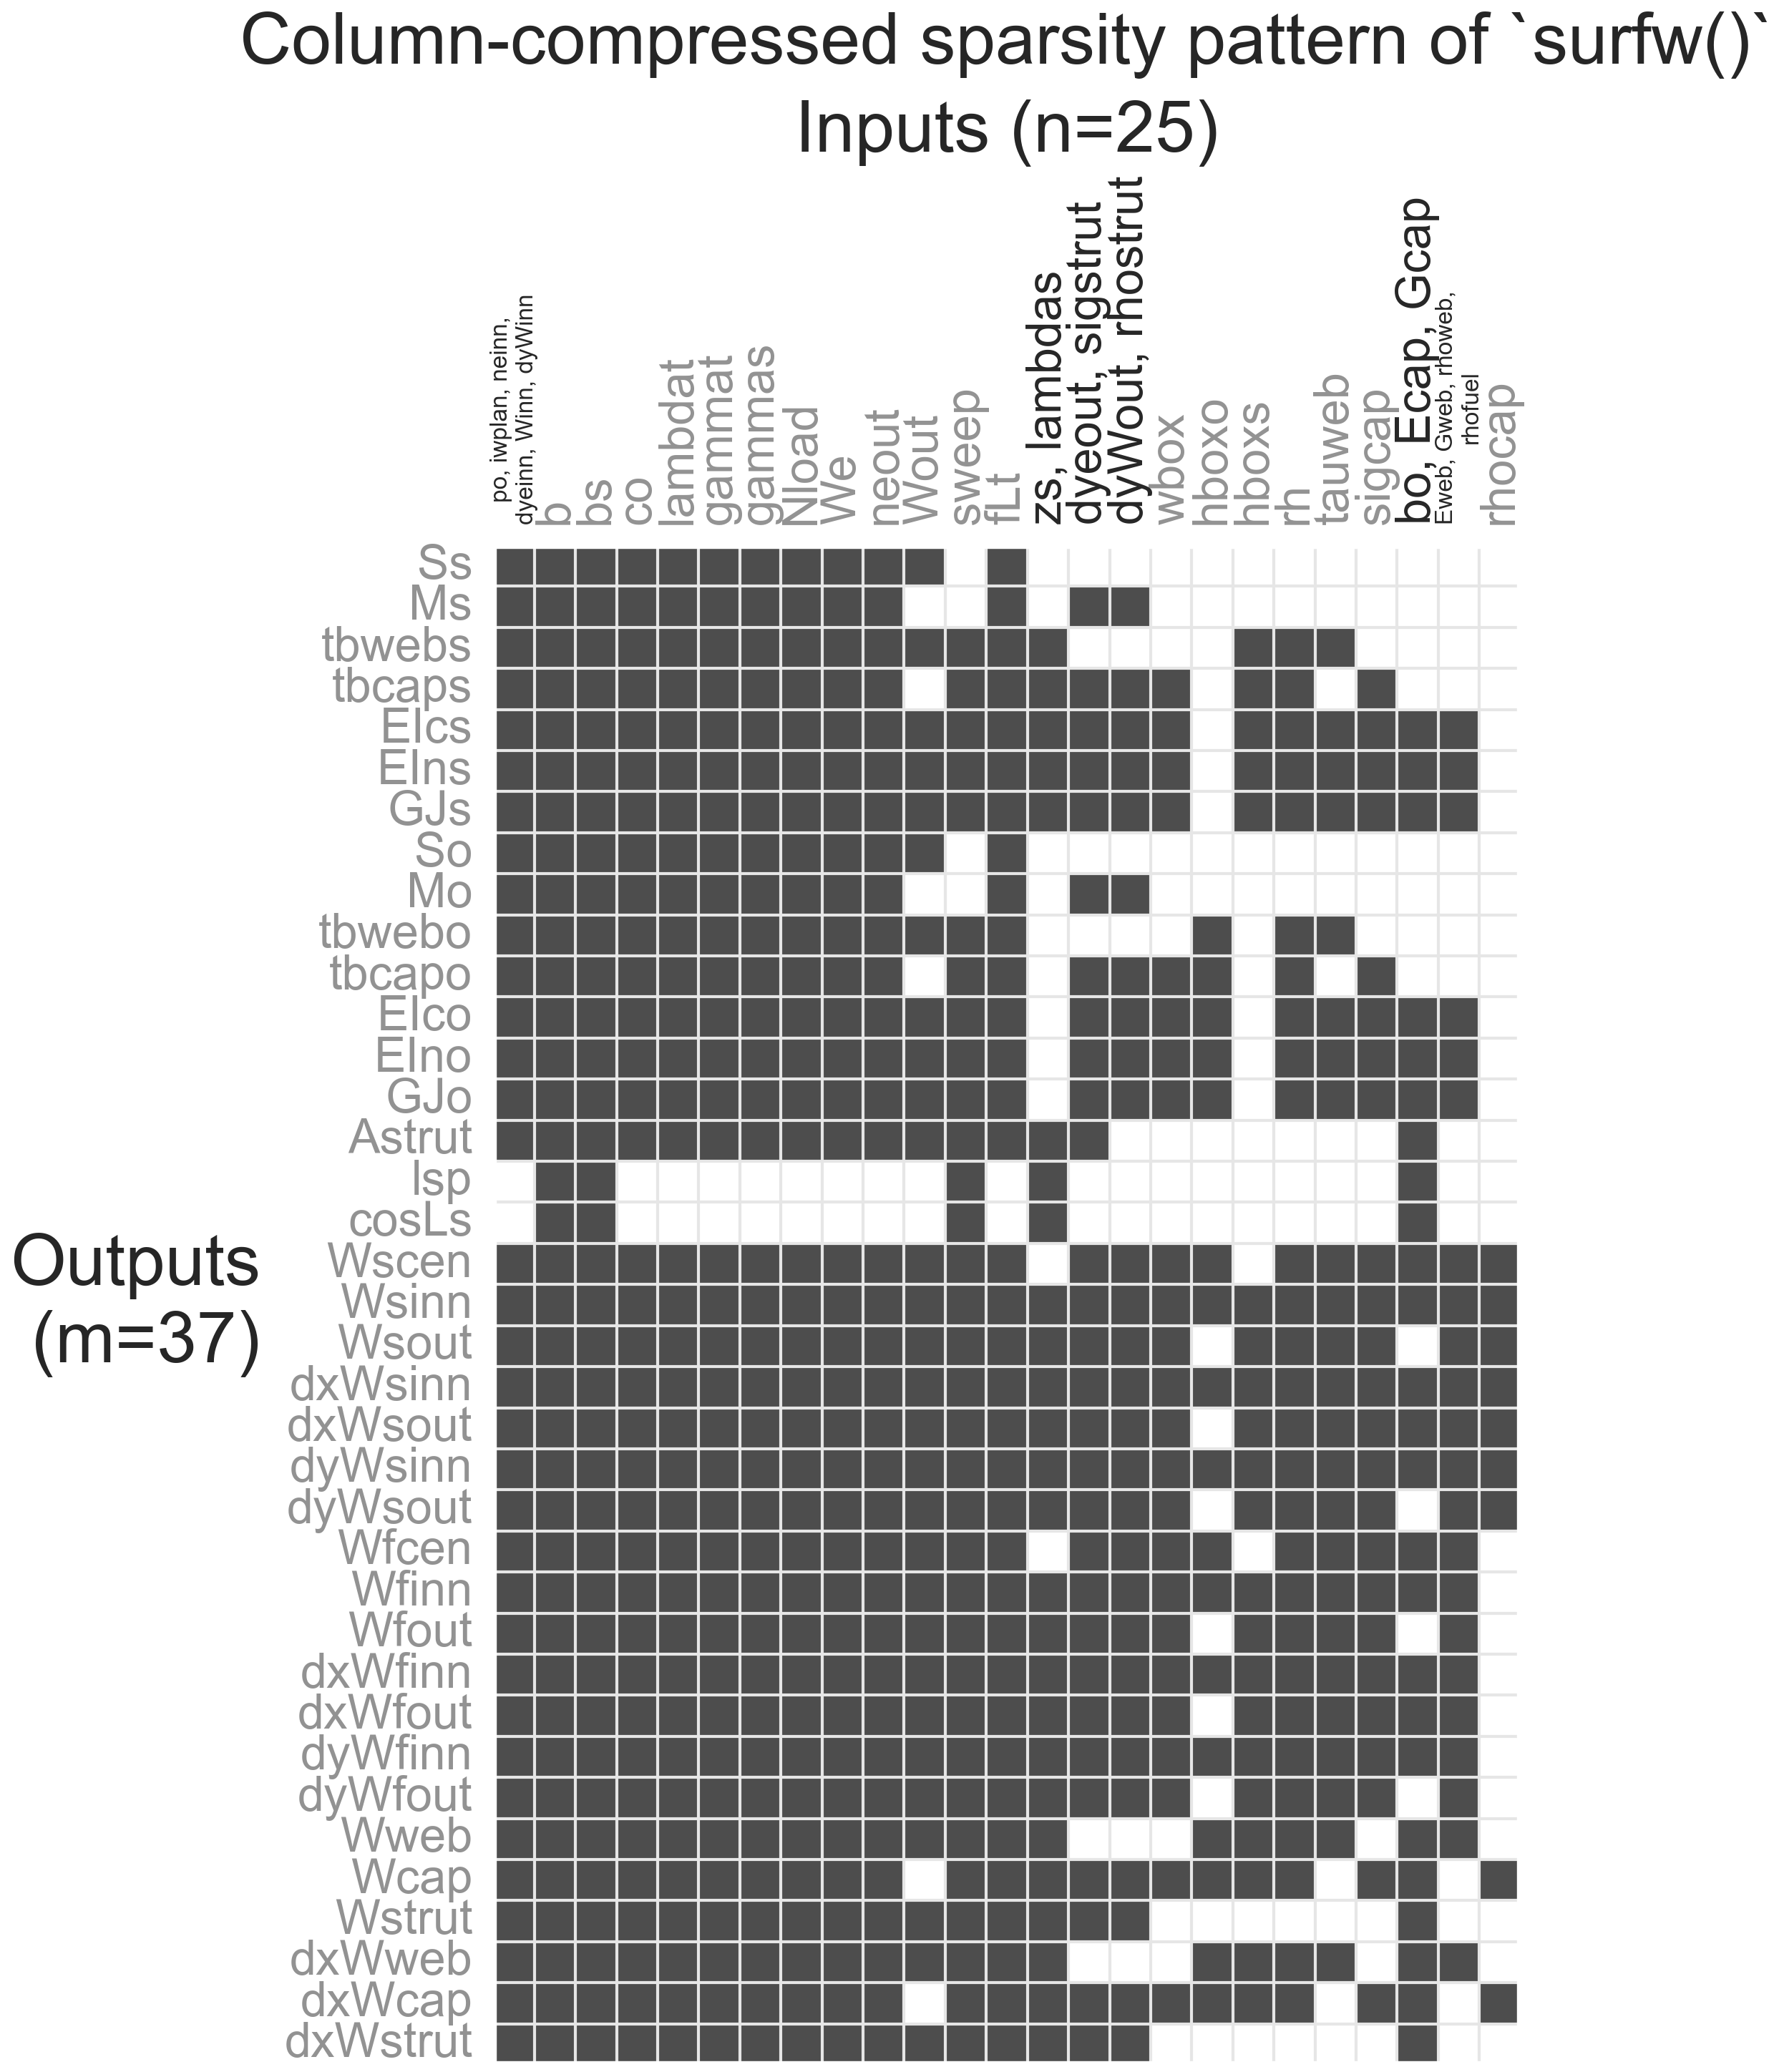
\includegraphics[width=5in]{../figures/nan-propagation/image3-crop.png}
    \caption{Compressed sparsity pattern of the TASOPT wing weight model, obtained by applying vertex coloring to the sparsity pattern of Figure \ref{fig:nan-jacobian}.}
    \label{fig:nan-jacobian-compressed}
\end{figure}


\section{Speed Considerations}

This gradient acceleration comes at a small upfront computational cost, since performing the sparsity trace requires a number of function evaluations equal to the number of inputs. This is true for both existing methods (described in Section \ref{sec:nan-existing-methods}) and for NaN-contamination. This cost is nearly always worthwhile in the context of design optimization: for the TASOPT wing model, a sparsity trace ``pays for itself'' in runtime if the subsequent optimization process requires more than three gradient evaluations.

In some cases, the runtime of a NaN-contamination-based sparsity trace will be essentially equal to that of standard finite-difference-based sparsity estimate. Intuitively, this makes sense, because both approaches require the same number of black-box function evaluations. However, in other cases, NaN-contamination can actually be significantly faster due to operator \textit{short-circuiting}. In this context, short-circuiting refers to operators that will check for NaN input values before performing computation; if any are found, the computation is skipped and a NaN is immediately returned instead. Programming languages and math libraries vary widely in whether and how they implement NaN-short-circuiting, so the magnitude of this potential speed-up is highly case-dependent.

% TODO add examples?


\section{Potential Limitations}

While NaN-contamination eliminates a notable false-negative failure mode compared to existing methods, it also has several possible pitfalls that merit discussion. Some of these pitfalls are shared with existing methods, while others are unique to this technique.

\subsection{Mathematical False-Positives}

One limitation of NaN-contamination is that it can introduce new false-positive failure modes. To illustrate one possible mechanism, consider a scenario where we attempt to NaN-propagate through a black-box function written in code as $f(x)= x - x$. If $x$ is real-valued, then the correct result of a sparsity trace is that the input $x$ and the output $f(x)$ are structurally unrelated. However, a NaN-contamination technique will indicate a possible dependency here, as NaN values do not subtractively cancel. In contrast, existing gradient-based methods will correctly identify independence. More generally, this kind of false-positive can occur in any function where self-cancellation leads to structural independence, such as $f(x) = \sin(x)^2 + \cos(x)^2$ or $f(x) = x^0$.

In some ways, this false-positive is an unavoidable result of the same properties that allow NaN-contamination to eliminate false negatives due to coincidental zero gradients. In theory, global knowledge of this function as a computational graph could allow this self-cancellation to be detected and avoided. However, this would require a level of introspection that is fundamentally incompatible with the black-box nature of the function.

\subsection{Internal NaN Handling}

NaN-contamination is not compatible with all black-box functions. In particular, black-box functions that internally handle NaN values may not allow propagation. Most commonly in this scenario, the function will instead raise an error and halt the computation. This behavior is easily and immediately detected, and the sparsity detection routine can fall back to existing gradient-based methods in these cases.

A more serious failure mode can occur if the program actively overwrites NaN outputs, as this can result in false negatives in the sparsity trace. Fortunately, this overwriting behavior is quite rare in engineering analysis code today. The main way this can occur is if the black-box code returns special flag values (sometimes called \emph{magic numbers}) to signal invalid computation, though this is generally considered an anti-pattern and avoided in numeric code. Even in code that has this overwriting behavior upon seeing a NaN result, most codes will at least raise a warning to the user.


%This can occur in a variety of ways, such as by using a math library that does not follow the IEEE 754 standard, or by explicitly checking for NaN values and returning a non-NaN result. In these cases, NaN-contamination will not be able to propagate through the function, and the sparsity trace will fail. This limitation is usually easy to detect, as the function will return a non-NaN result when given a NaN input. In these cases, the user can fall back to existing methods.

% usually just fails to run; that's ok

% Informally: it's rare that engineering code will perform a calculation and simply ignore any NaNs that result (as opposed to raising an error, or at least a warning)

\subsection{Branching Code Execution}

Finally, branching code execution remains a challenge for NaN-contamination-based sparsity tracing, just as it is with existing methods. An example of this can be shown with the wing weight demonstration problem described in Section \ref{sec:nan-demo}. Here, the input variable \texttt{iwplan} controls the wing configuration. Specifically:

\begin{itemize}[noitemsep]
    \item \texttt{iwplan = 0} or \texttt{iwplan = 1} corresponds to a cantilever wing with no strut.
    \item All other values of \texttt{iwplan} correspond to a wing with a strut.
\end{itemize}

Perhaps unsurprisingly, the sparsity pattern is materially different if you change the wing configuration by adding a struct. This is shown in Figure \ref{fig:nan-jacobian-branching}.

% subfigure setup; a) has no strut, b) has a strut
\begin{figure}[H]
    \centering
    \begin{subfigure}{0.45\textwidth}
        \centering
        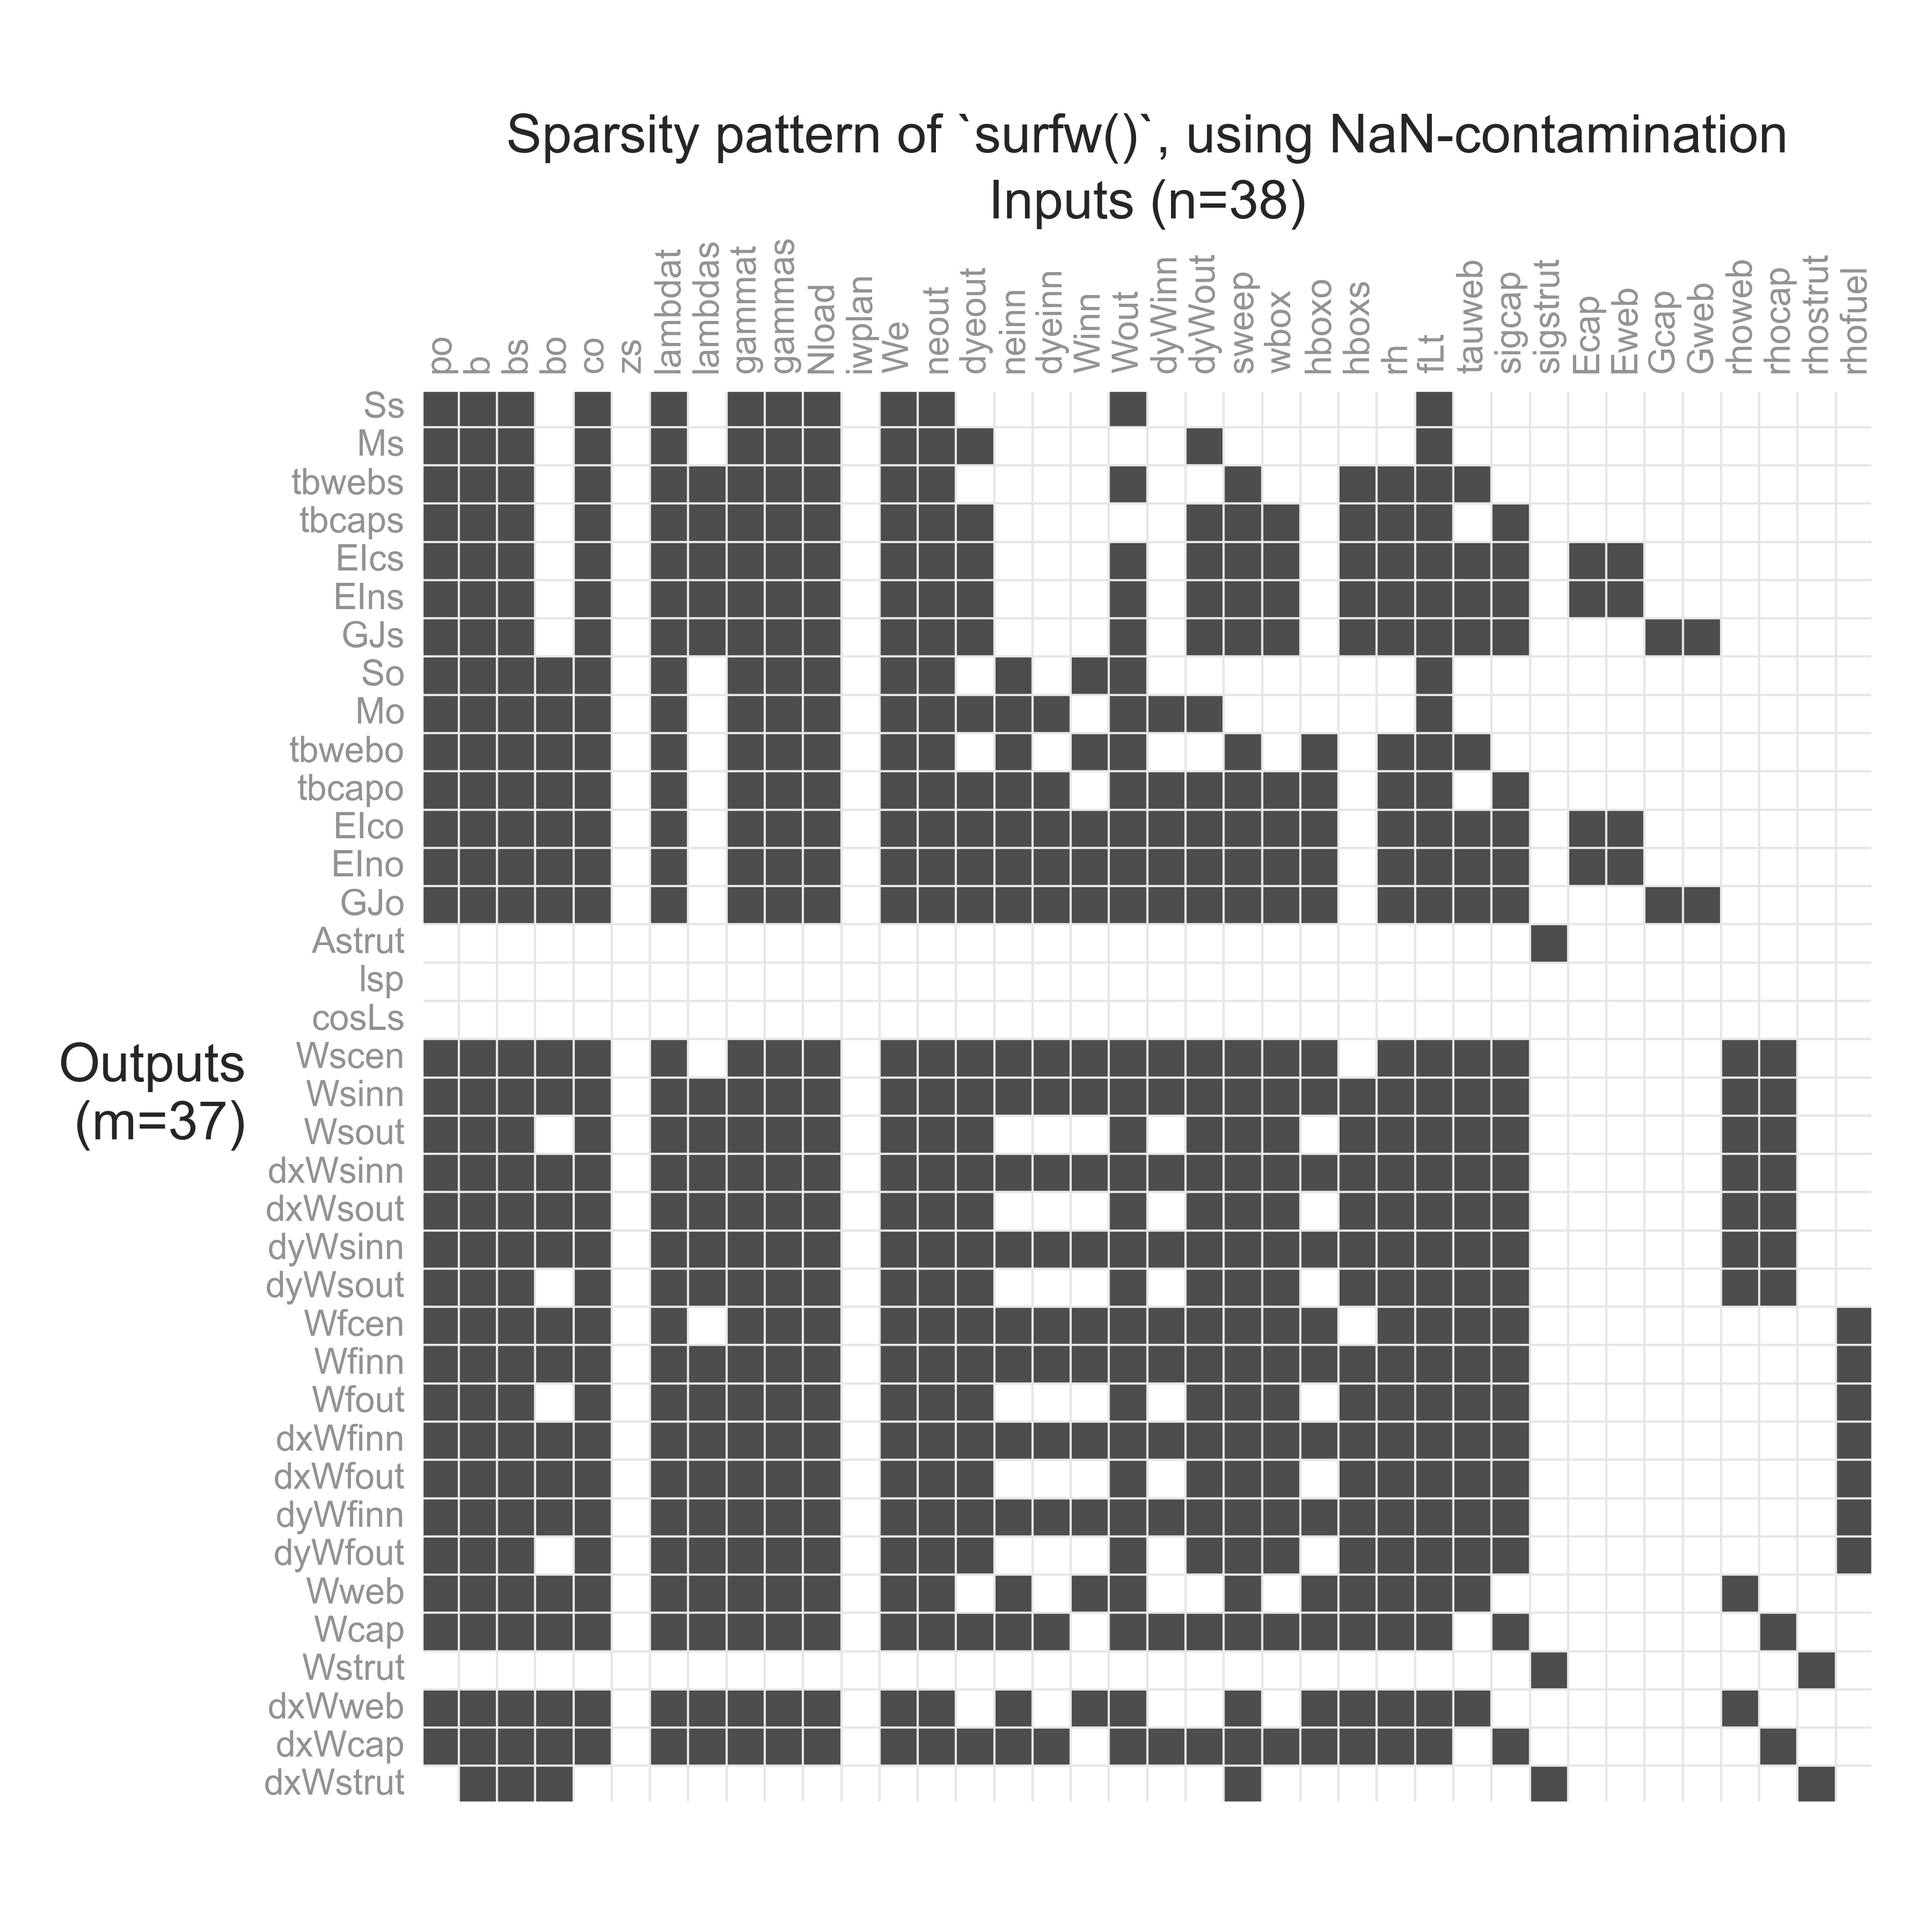
\includegraphics[width=2.5in]{../figures/nan-propagation/image4.png}
        \caption{Sparsity pattern with no strut}
    \end{subfigure}
    \begin{subfigure}{0.45\textwidth}
        \centering
        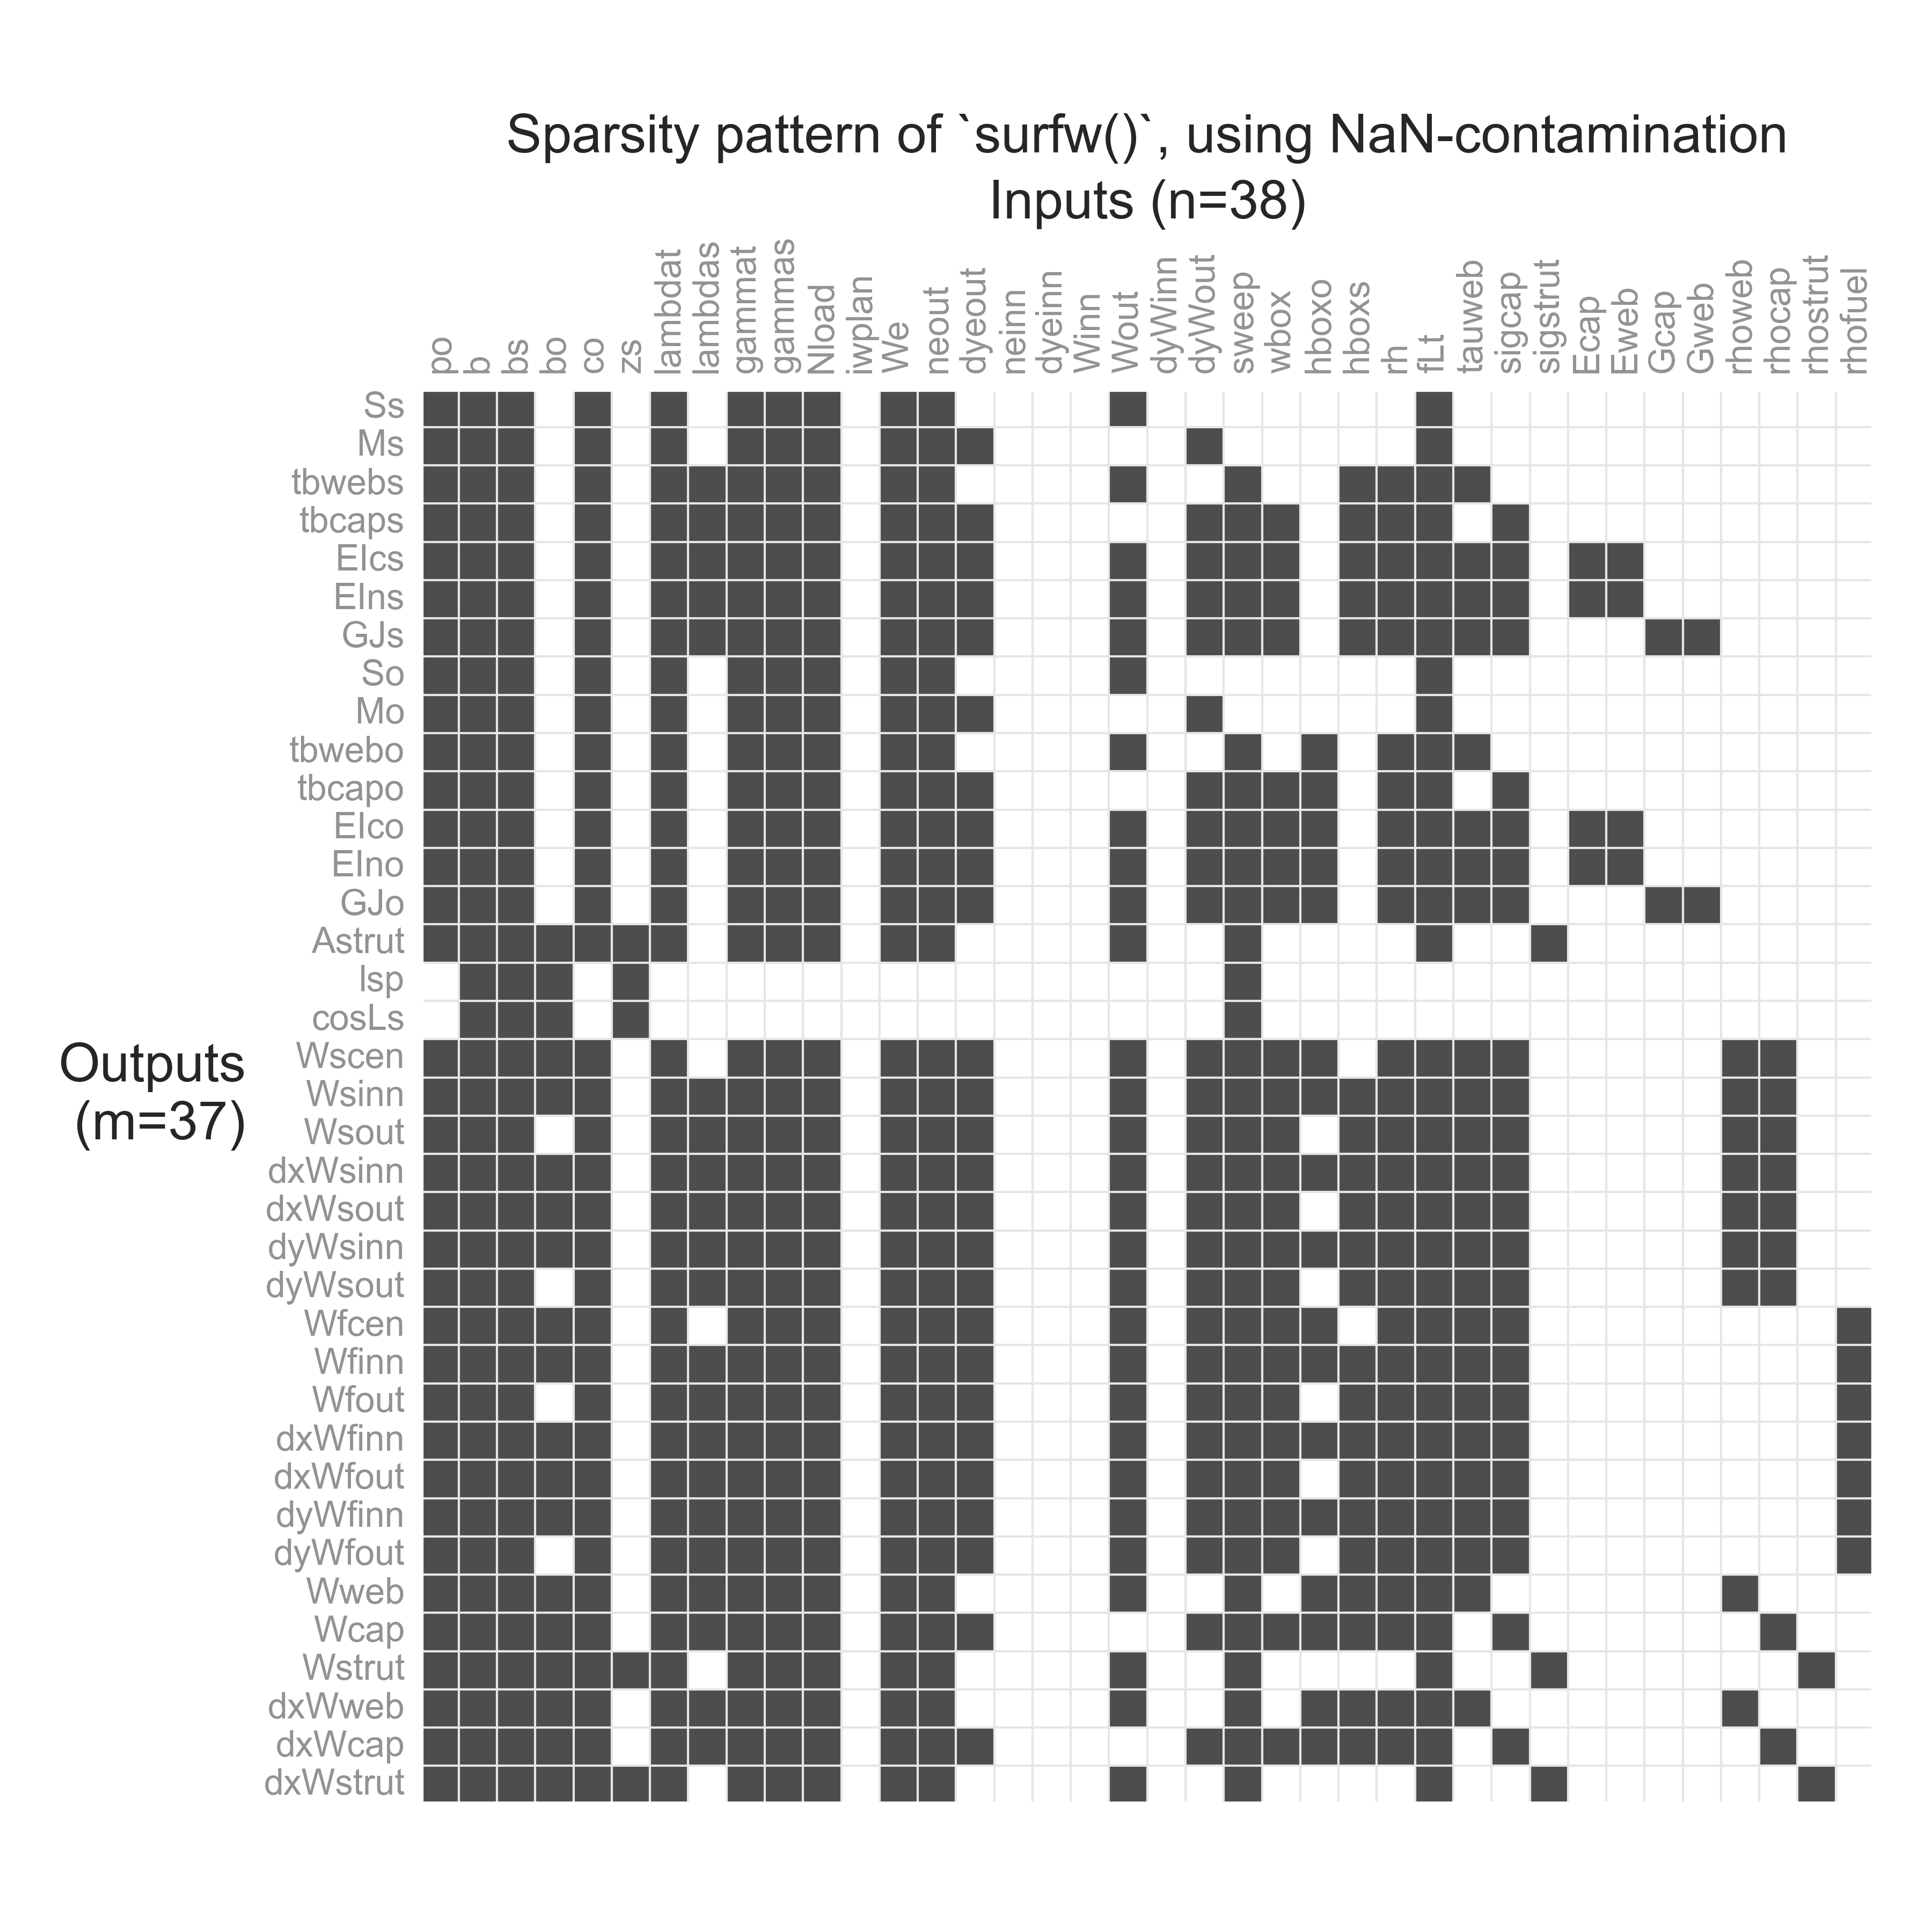
\includegraphics[width=2.5in]{../figures/nan-propagation/image5.png}
        \caption{Sparsity pattern with a strut}
    \end{subfigure}
    \caption{Sparsity pattern of the TASOPT wing weight model, estimated using NaN propagation, with and without a strut.}
    \label{fig:nan-jacobian-branching}
\end{figure}

% TODO talk about false-positive in vectorized operations (e.g., matmul contaminating entirely)


\section{Mitigating Branching Code Execution}


\section{Advanced Strategies}

\subsection{Chunking}

Further accelerations are possible. One novel proposed acceleration, which we term ``chunking'', seeds multiple adjacent elements of the input vector with NaN values simultaneously. As an example: if pairs of adjacent inputs are seeded, this has the benefit of halving the number of function calls, at the detriment of providing overly-conservative sparsity information\footnote{as one cannot determine which NaN input caused a given output to return NaN, so neither can be ruled out}. This exploits the fact that a conservative sparsity pattern can still provide a significant speedup, depending on the sparsity pattern. It also exploits the fact that human-written code tends to have a high degree of locality\footnote{in other words, humans tend to code Discipline A in its entirety before implementing analyses for Discipline B} (e.g., inputs 10 and 11 are much more likely to share a sparsity pattern than inputs 10 and 100), and hence these chunked sparsity patterns can be surprisingly accurate in practice. Thus, chunking may offer significant practical speedups by exploiting typical problem structure; a computational analogy would be how an $A^*$ graph traversal algorithm outperforms Dijkstra's algorithm in practice despite identical worst-case complexity. This and other heuristics can significantly reduce the number of black-box function evaluations required to trace the sparsity pattern.

\subsection{NaN Payload Encoding}

% TODO Encoding of NaN source information into payload? `manual_bit_banging.py`

There are several subtleties to address for robustness across numerical code. First, some functions may internally handle NaN values via exceptions, preventing contamination and hence precluding this strategy. However, NaN propagation is common in most numerical libraries. Second, conditional logic can complicate tracing, but most libraries propagate NaNs through static conditional statements (i.e., a flattened if-else statement where both branches are fused). Overall, NaN propagation shows promise for automated sparsity detection through common black-box functions. Integrating this technique into the code transformation paradigm could expand its applicability.
